\documentclass[11pt,a4paper]{article}

\usepackage[margin=22mm]{geometry}
\usepackage{amsmath}
\usepackage{booktabs}
\usepackage{graphicx}
\usepackage[hidelinks]{hyperref}
\usepackage{microtype}
\usepackage[section]{placeins}
\usepackage{tabularx}
\usepackage{xcolor}
\usepackage[font=small,labelfont=bf]{caption}

% All report figures are authored at the final 166 mm text width.
\graphicspath{{figures/}{../figures/}}
\setlength{\parindent}{0pt}
\setlength{\parskip}{0.55em}
\renewcommand{\arraystretch}{1.18}

\title{\textbf{Resolution and MPI scaling for multiphase flows}}
\author{Vatsal Sanjay\\
\small Computational Multiphase Physics (CoMPhy) Lab\\
\small Department of Physics, Durham University\\
\small \url{https://comphy-lab.org/}}
\date{September 2026}

\begin{document}
\maketitle

\begin{abstract}

We study the CPU scaling of Basilisk for the stock Poisson and Laplacian
tests, Marangoni-driven migration, bubble bursting, elastic Taylor--Culick
retraction and drop impact. The measurements on MareNostrum~5 and Snellius
extend to 16,384 MPI ranks for the stock kernels. For Marangoni migration,
we also compare the drop velocity with its analytical value and find that
the error does not decrease monotonically at the finer resolutions.
At fixed resolution, the wall time initially decreases with increasing
rank count, then levels off and can increase again. The location of this
knee changes with the mesh and the flow being calculated. In a research
project, we first establish the resolution needed for the physical quantity
of interest, then use a scaling test to choose ranks near the knee.
Grid independence at one set of parameters cannot be assumed at another,
nor can the rank count chosen for one mesh be assumed suitable after
refinement. Both tests need to be repeated as the parameter study develops,
particularly where smaller length scales or new flow regimes appear.
The same applies to regularizations and cutoffs introduced when solving
the continuum equations. A change in the numerical model or computing
system also requires a new scaling test.

\end{abstract}

\section{Grid sensitivity and parallel scaling}

A grid-independence study must follow the flow far enough to test the
quantity of interest. During bubble bursting, the cavity can collapse into
a jet much thinner than the bubble radius. Similarly, a drop that is well
resolved before impact can spread into a poorly resolved lamella. A mesh
chosen from the initial geometry alone may miss these later stages.
Moreover, convergence of the drop trajectory need not imply convergence of
the peak impact force or of a jet radius. The required resolution depends
on which of these quantities we calculate and how accurately we need it.

The grid is only one of the choices made when we solve the continuum
Cauchy equations numerically. We also choose the time-step restriction,
solver tolerances and domain size, and may regularize a constitutive law
or introduce a cutoff. In a regularized viscoplastic model, the effective
viscosity may be capped at a finite value. The nominally unyielded region then has a large but finite
viscosity. Refinement at a fixed cap tests convergence for that regularized
equation; the viscosity cap must be varied separately.
The criterion used to identify flow arrest needs a similar check. We tested
both in our study of bursting bubbles in a viscoplastic
medium~\cite{sanjay2021-bursting}. Even after these numerical tests,
comparison with theory and experiments is needed to assess the physical
predictions of the model.

These checks cannot be settled for an entire project by testing one case
at the outset. A change in the physical parameters can produce a thinner
jet, steeper gradients or a different flow regime, for which the same mesh
is insufficient. Increasing the resolution also changes the amount of work
assigned to each MPI rank. Once we have established an adequate resolution,
we therefore measure the wall time at several rank counts. We seek the
\emph{knee}, where the curve bends from approximately inverse scaling
towards a plateau. Around this bend, doubling the rank count no longer
halves the wall time. Its location must be checked again as the calculation
changes.

\section{Numerical method and timing}

For each strong-scaling test, we vary the number of MPI ranks
$N_{\mathrm{MPI}}$ while keeping the grid resolution, geometry, material
parameters and output settings fixed. We use uniform grids with the
Basilisk tree backend and disable mesh adaptation during these timings.
The plots give wall time per iteration; $T\propto N_{\mathrm{MPI}}^{-1}$
denotes ideal scaling. The separate Marangoni accuracy study uses mesh
adaptation.

We use the stock Poisson and Laplacian tests without
modification~\cite{basilisk-mpi-circle,basilisk-mpi-laplacian}, taking the
mean time per kernel operation over each test's timing loop, together with
the time spent in MPI routines.
For retraction and impact, the timer covers ten solver steps after
geometric initialization. The bursting case starts from an interface
constructed separately, and the ten-step timer begins after restoring it.
Neither construction nor restoration enters this time. Checkpoint output is
disabled for all three cases. When selecting ranks for a full simulation,
we also need timings from the relevant stages of the flow with the output
that the simulation will write.

For Marangoni migration, we divide the elapsed solver time by the number
of steps in the prescribed interval. At 256 points per radius, the interval
is $t/t_0=0$--$0.05$ for 2--256 ranks and $0$--$0.5$ for 512--1,024 ranks.
Thus the averages on either side of this change cover different flow
histories.

Each configuration has been timed once. The curves identify where scaling
improves or deteriorates, but neighbouring points on a nearly flat curve
should be repeated before choosing between them. The code, timing tables
and plotting scripts are available at
\url{https://github.com/comphy-lab/hpc-basilisk-scaling}. To compare runs
between systems, we record the source revision, compiler flags and MPI
implementation, together with the node type, ranks per node and rank
binding.

\section{Poisson and Laplacian tests}

In an incompressible-flow calculation, the velocity obtained after
advection, viscous stresses and interfacial forces must be projected onto
a divergence-free field. Basilisk uses a multigrid Poisson solver for this
step. Restriction and prolongation connect the different grid levels, and
MPI communication exchanges data between subdomains. At a fixed grid
size, each rank has fewer cells as the number of ranks increases, while
these exchanges are still required. The stock tests measure the resulting
scaling before interface reconstruction or constitutive evolution is added.

For the two-dimensional test, we use a full quadtree at $L=14$, containing
$2^{28}$ cells. The Snellius Poisson time decreases up to 8,192 ranks and
levels off at 16,384 ranks (Figure~\ref{fig:kernel-scaling}(a)). As the
wall time approaches this plateau, communication takes a larger fraction
of it. We include the published Curie data for comparison with the same
test.

\begin{figure}[htbp]
  \centering
  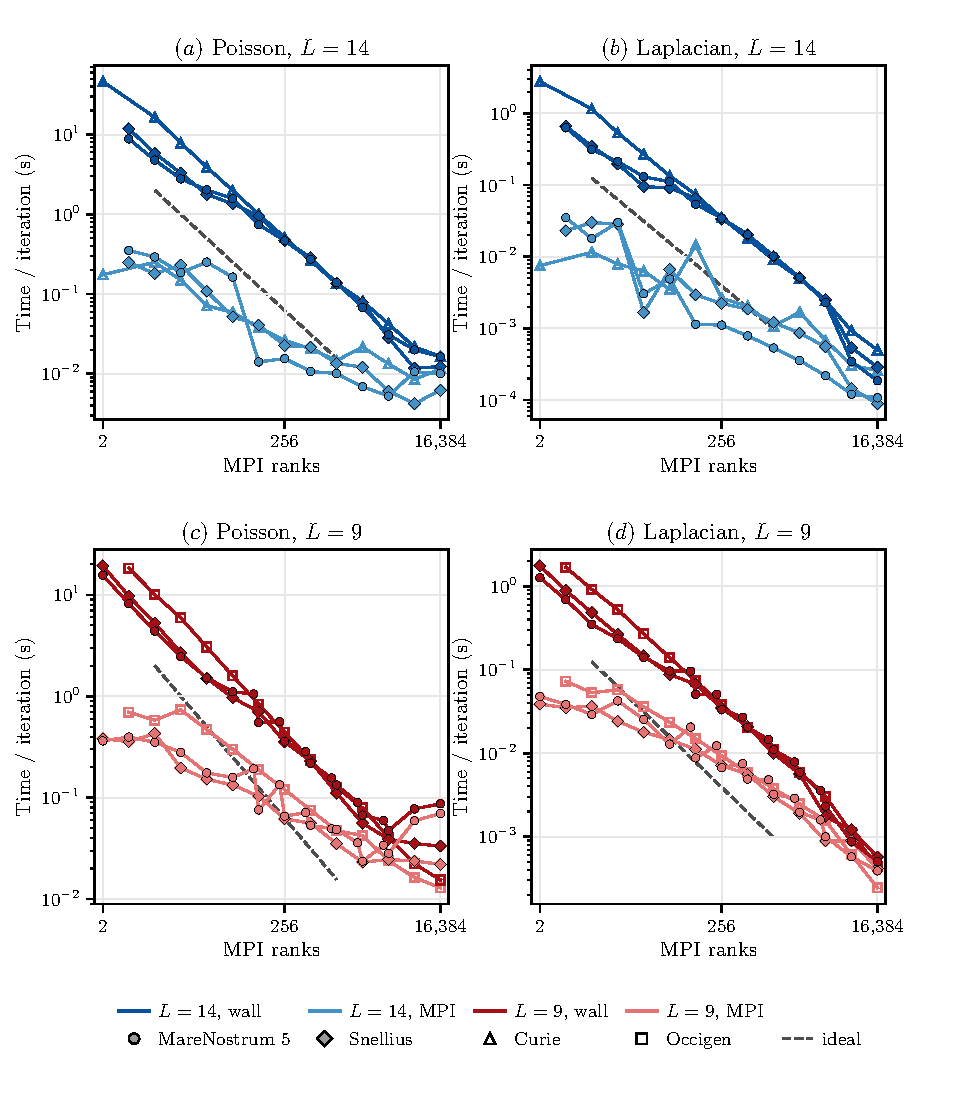
\includegraphics[width=\textwidth]{kernel-scaling-combined-report.pdf}
  \caption{Time per iteration for the stock Poisson (left) and Laplacian
  (right) tests. (a,b) Full two-dimensional quadtree at $L=14$.
  (c,d) Full three-dimensional octree at $L=9$. The $L=14$ results are
  shown in blue and the $L=9$ results in red, with darker shades for wall
  time and lighter shades for MPI time. Circles denote MareNostrum~5 and
  diamonds Snellius. The open symbols are the published Curie
  (two-dimensional) and Occigen (three-dimensional) data. Solid lines join
  the measured points. The grey dashed segments at the lower left and upper
  right show $T\propto N_{\mathrm{MPI}}^{-1}$; their vertical
  positions are arbitrary.}
  \label{fig:kernel-scaling}
\end{figure}

The three-dimensional test uses a full octree at $L=9$, with $2^{27}$
cells, and is compared with the published Occigen data. On Snellius, the
Poisson time decreases from $19.34$~s at two ranks to $0.0390$~s at
4,096 ranks. Increasing to 16,384 ranks reduces it to $0.0333$~s
(Figure~\ref{fig:kernel-scaling}(c)). Thus four times as many ranks save
only about 15\% of the wall time over this interval. The Laplacian takes less time per iteration on the
same grid, and its curve has a different dependence on the rank count.

\section{Marangoni migration}

Here, the drop moves under a prescribed surface-tension gradient. We use
the conservative, balanced formulation of Abu-Al-Saud, Popinet and
Tchelepi~\cite{abu-al-saud2018}. The analytical migration velocity gives us
a reference against which to test the calculated drop speed as the mesh
is refined.

Figure~\ref{fig:application-scaling} shows the timings for two series of
calculations. In the axisymmetric case, we increase the resolution from
64 to 512 points per drop radius. In the planar case, we increase the
number of drops from one to 32, keeping 64 points per radius. Both series
extend to 1,024 ranks. The curves for the smaller calculations flatten
while the larger ones still decrease. Increasing either the resolution or
the number of drops changes how much computation can be distributed over
the MPI ranks. A rank count near the plateau of a coarse single-drop case
can still lie on the decreasing part of a finer-grid or multiple-drop curve.

\begin{figure}[htbp]
  \centering
  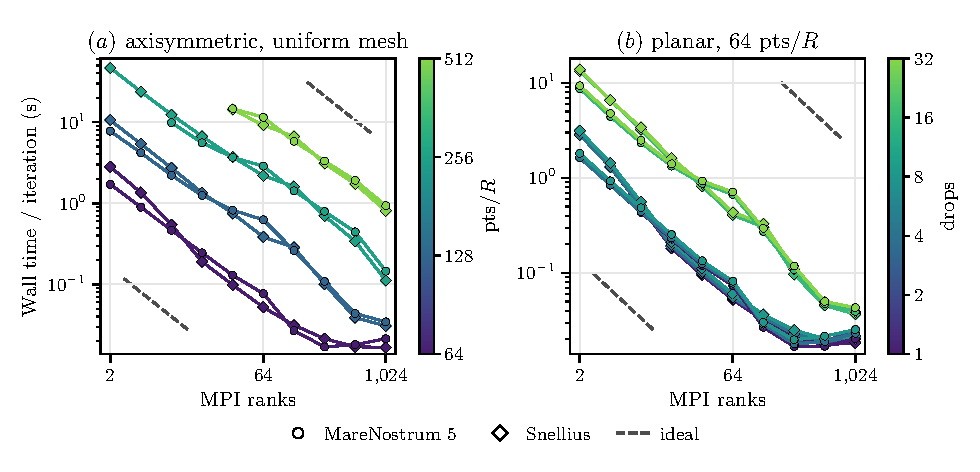
\includegraphics[width=\textwidth]{marangoni-uniform-ndrop-per-iter-report.pdf}
  \caption{Wall time per solver step for Marangoni-driven migration on
  MareNostrum~5 GPP (circles) and Snellius Genoa (diamonds).
  (a) Axisymmetric calculations with 64--512 points per drop radius.
  (b) Planar calculations with 1--32 drops, each resolved by 64 points per
  radius. The dashed lines give the ideal scaling. For integral
  surface-tension formulations applied to Marangoni flow, see
  Ref.~\cite{saini2025-marangoni}.}
  \label{fig:application-scaling}
\end{figure}

We compare the migration velocity with the Young--Goldstein--Block
prediction and the Basilisk reference data in Figure~\ref{fig:validation}.
The relative error decreases rapidly between eight and 32 points per
radius. Beyond 32 points per radius, it varies non-monotonically with
refinement. The $N^{-2}$ line is a guide for the coarse-grid points; fitting
this slope through all the resolutions would obscure the change in
behaviour at the finer grids. The drop-frame velocity fields show the
flow developing during migration.

Although the larger grids scale over more ranks, they do not give a
monotonic reduction in the velocity error. Domain size, integration time
and solver tolerance are other possible sources of error and need separate
tests. We cannot infer accuracy from the improvement in parallel scaling.

\begin{figure}[htbp]
  \centering
  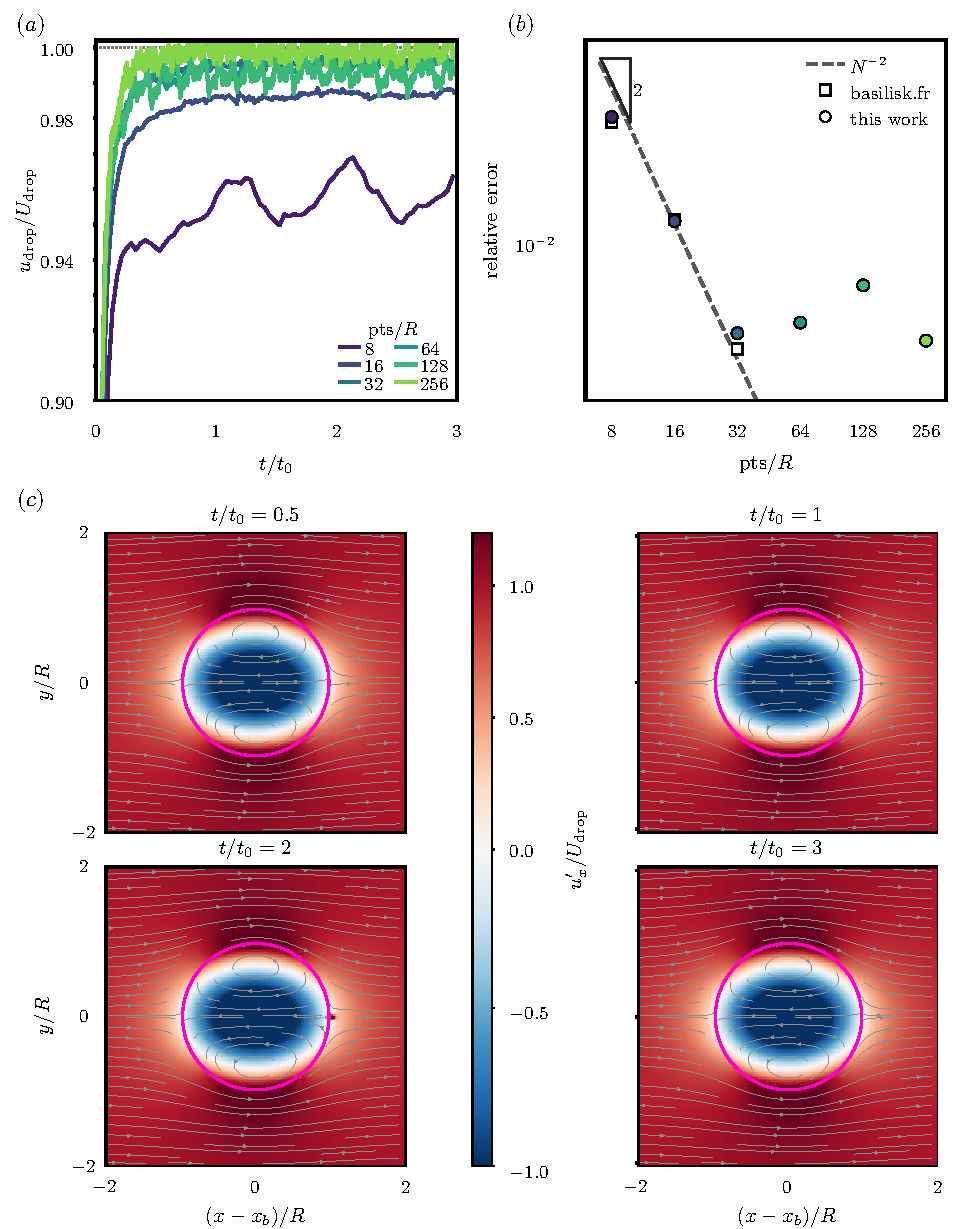
\includegraphics[width=\textwidth]{marangoni-validate-vt-fields-report.pdf}
  \caption{Marangoni-driven migration under a prescribed surface-tension gradient.
  (a) Speed relative to the Young--Goldstein--Block prediction at 8--256
  points per radius. (b) Relative error and an $N^{-2}$ guide.
  (c) Drop-frame axial velocity at 64 points per radius, shown at
  $t/t_0=0.5$, $1$, $2$ and $3$. Magenta marks the interface. See
  Ref.~\cite{saini2025-marangoni} for the interfacial-stress formulation.}
  \label{fig:validation}
\end{figure}

\section{Bursting, retraction and impact}

We next consider bubble bursting, elastic Taylor--Culick retraction and
Newtonian drop impact, using the same two-phase solver infrastructure.
The three axisymmetric cases use $L=9$, $10$ and $11$, corresponding to
$512^2$, $1024^2$ and $2048^2$ cells. The coarser grids are tested over
2--768 ranks. At $L=11$, the tests start at eight ranks and reach 768
ranks for bursting and 2,304 ranks for retraction and impact.

At $L=10$, the three cases have similar scaling ranges despite their
different times per step (Table~\ref{tab:axisymmetric-times}). On the
coarser $L=9$ grid, the time for bursting levels off at about $0.008$~s
beyond 96 ranks, while retraction and impact approach $0.010$~s and
$0.011$~s, respectively. Refinement changes this range. The same rank
count can consequently fall on a decreasing part of one curve and near
the plateau of another, depending on both the mesh and the flow being
calculated.

\begin{table}[htbp]
\centering
\small
\begin{tabular}{@{}lrrr@{}}
\toprule
& \multicolumn{3}{c}{Wall time per iteration (s), $L=10$} \\
\cmidrule(l){2-4}
Kernel & 2 ranks & 192 ranks & 768 ranks \\
\midrule
Bursting bubble & 1.28 & 0.0174 & 0.0108 \\
Elastic Taylor--Culick & 1.85 & 0.0231 & 0.0127 \\
Newtonian drop impact & 2.04 & 0.0267 & 0.0173 \\
\bottomrule
\end{tabular}
\caption{Wall time per iteration on Snellius Genoa for the three
axisymmetric cases.}
\label{tab:axisymmetric-times}
\end{table}

For the finest bursting case, the time decreases to $0.0407$~s per step at
384 ranks and then rises to $0.0781$~s at 768 ranks
(Figure~\ref{fig:bursting-uniform}). Doubling the number of ranks nearly
doubles the time in this part of the curve. The elastic sheet includes
log-conformation extra-stress evolution and continues to become faster
over the larger rank range: the $L=11$ time falls from $0.0341$~s at
768 ranks to $0.0193$~s at 1,536 ranks and $0.0152$~s at 2,304 ranks
(Figure~\ref{fig:taylorculick-uniform}). The final increase in ranks still
reduces the time, although by a smaller amount than the preceding one.

For Newtonian impact, the drop is initially at $(1.05,0)$ in a box of
side~8, moving towards the left wall, with the axis of symmetry along the
bottom boundary. At $L=11$, we obtain $0.0339$~s per step at 768 ranks,
$0.0250$~s at 1,536 ranks and $0.0423$~s at 2,304 ranks
(Figure~\ref{fig:drop-impact-uniform}). Hence, increasing the rank count
from 1,536 to 2,304 helps the retraction calculation but slows the impact
calculation. The largest rank count reached by a test is not necessarily
a useful one for that flow. These application timings do not separate
computation, communication and other overheads, so they do not determine
which contribution causes the departure from ideal scaling.

The sequences in Figures~\ref{fig:bursting-uniform}--\ref{fig:drop-impact-uniform}
are from separate completed simulations. They show the narrowing cavity
and emerging jet, the growing rim of the retracting sheet, and the thin
lamella produced by drop impact. A resolution study must include these
stages if the jet, rim or lamella determines the result of interest.
Within each sequence, the spatial scale and colour normalization are fixed.
The frames are ordered from left to right, then top to bottom.

\begin{figure}[p]
  \centering
  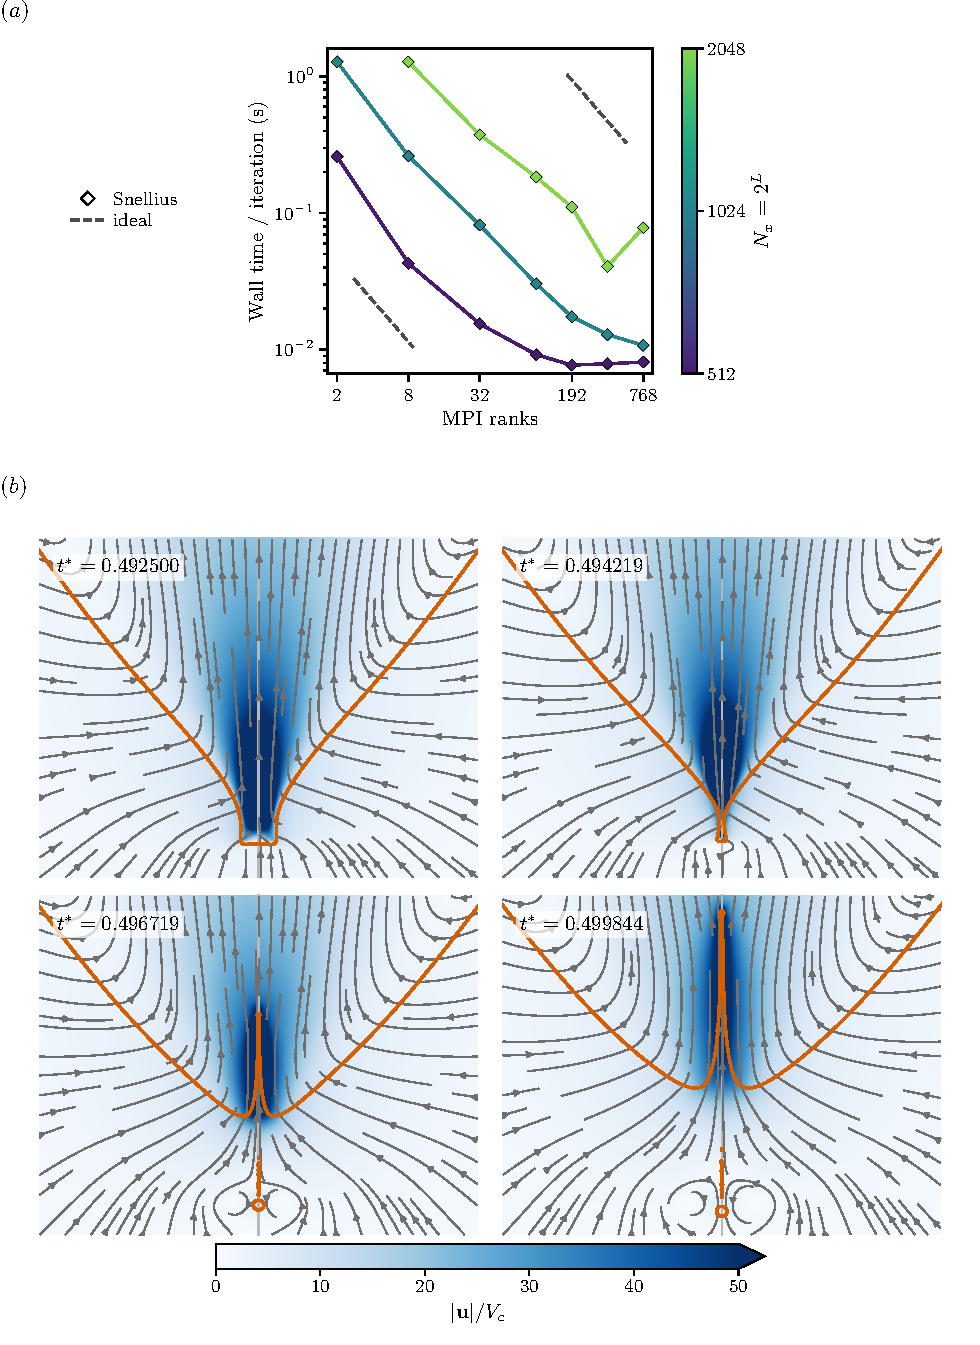
\includegraphics[width=\textwidth]{bursting-uniform-illustrated.pdf}
  \caption{Bursting bubble~\cite{dixit2025-bursting,sanjay2021-bursting}.
  (a) Snellius Genoa strong scaling of the
  axisymmetric calculation; colour gives $N_x=2^L$ and dashed
  lines show ideal scaling. (b) Jet inception~\cite{gordillo2026-jets}
  at $Oh=0.03$, $Bo=0$.
  Blue gives $|\boldsymbol{u}|/V_c$, where
  $V_c=\sqrt{\sigma/(\rho_l R)}$ and $t^*=tV_c/R$; grey curves are
  instantaneous streamlines and orange marks the interface. The sequence
  shows the narrowing cavity, emerging jet and entrapped bubble.
  Colours saturate above $50V_c$.}
  \label{fig:bursting-uniform}
\end{figure}

\begin{figure}[p]
  \centering
  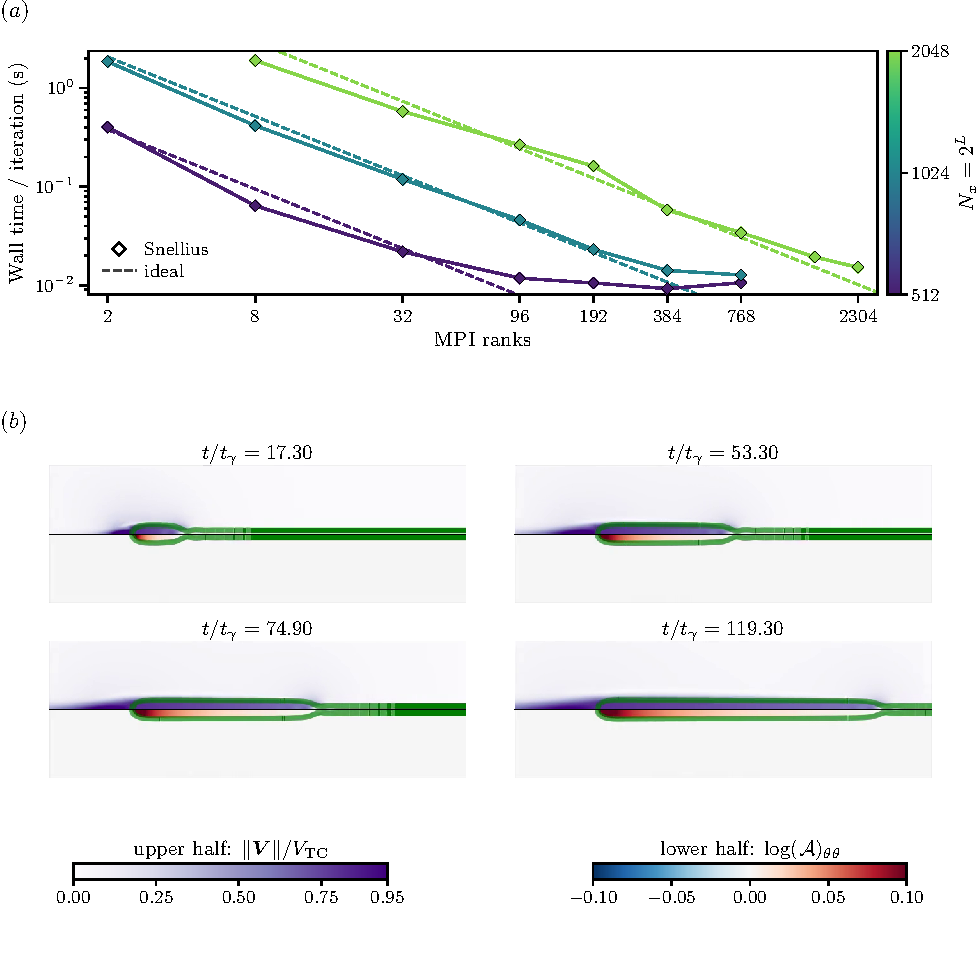
\includegraphics[width=\textwidth]{taylorculick-uniform-illustrated.pdf}
  \caption{Elastic Taylor--Culick retraction. (a) Snellius Genoa strong
  scaling of the axisymmetric calculation.
  (b) Rim evolution at $Ec=0.1$, $Oh=0.05$ in a relaxation-free calculation.
  The view follows the rim. Each frame combines speed relative to the
  Taylor--Culick velocity (upper half) and the azimuthal log-conformation
  $(\log\mathcal{A})_{\theta\theta}$ (lower half); green marks the
  interface. Here $t_\gamma=\sqrt{\rho H_0^3/\sigma}$, with $H_0$ the
  initial sheet thickness. For retraction and the influence of the
  surroundings, see Ref.~\cite{sanjay2022-taylorculick}.}
  \label{fig:taylorculick-uniform}
\end{figure}

\begin{figure}[p]
  \centering
  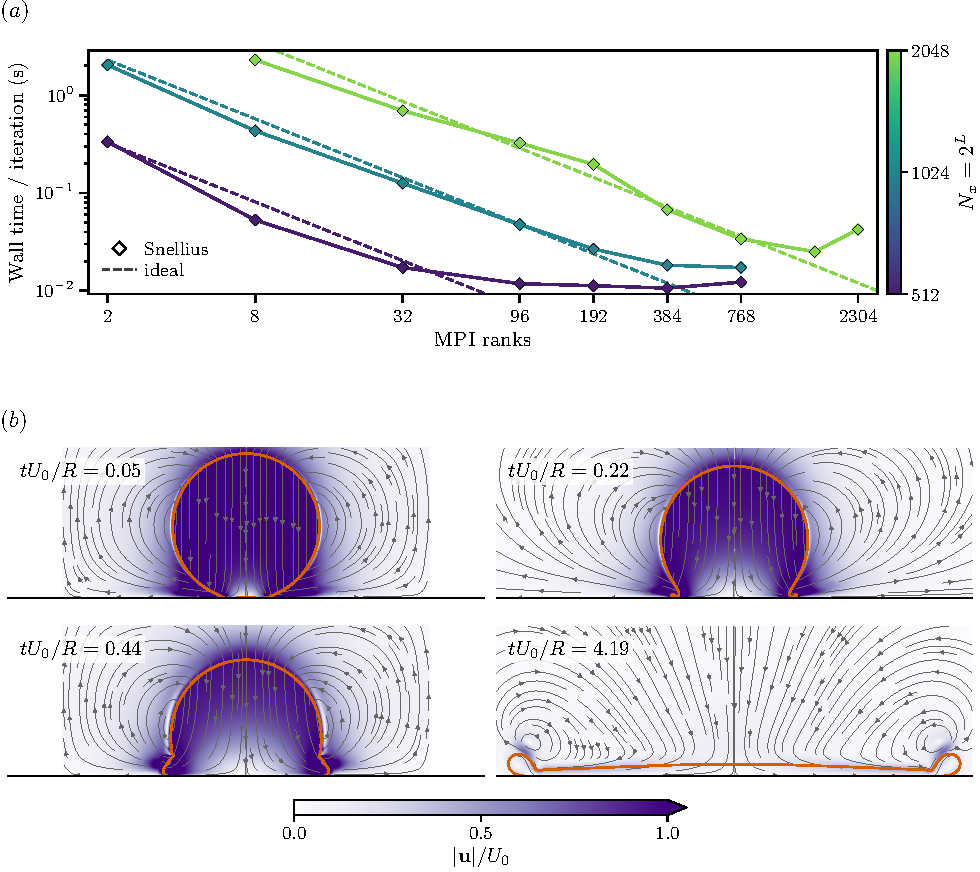
\includegraphics[width=\textwidth]{drop-impact-uniform-illustrated.pdf}
  \caption{Newtonian drop impact. (a) Snellius Genoa strong scaling of
  the axisymmetric calculation.
  (b) Impact and spreading at diameter-based $We_D=200$ and $Oh_D=0.01$.
  Lengths are scaled by the initial drop radius $R$ and time by $R/U_0$,
  where $U_0$ is the impact speed. Purple shows speed, grey curves are instantaneous streamlines,
  orange marks the interface and black marks the substrate.
  Colours saturate above $U_0$. All four frames retain the same view,
  including the extended lamella at $tU_0/R=4.19$. Related studies address
  free-surface wave focusing~\cite{kayal2025-focussing} and drop-impact
  forces and spreading~\cite{sanjay2025-impact,zhang2022-impact}.}
  \label{fig:drop-impact-uniform}
\end{figure}

\section{Choosing resolution and MPI ranks}

We prefer to run near the knee because the time saved by further
increasing the number of ranks becomes small. The shortest wall time can
still be useful for an urgent calculation, but for a parameter study those
additional cores may be better used to run another case. We quantify the
resource use by the allocated core time. If $C_{\mathrm{alloc}}$ cores
are reserved for a wall time $t_{\mathrm{wall}}$, then
\begin{equation}
  \mathcal{C}=C_{\mathrm{alloc}}\,t_{\mathrm{wall}}.
\end{equation}
Here $C_{\mathrm{alloc}}$ counts all reserved cores, including any that
remain idle. It equals $N_{\mathrm{MPI}}$ when each allocated core runs
one rank. If the scheduler reserves whole nodes, leaving some of their
cores idle does not reduce the allocation. We therefore compare both wall
time and allocated core time when selecting ranks near the knee.

We start with a grid study for the physical quantity and accuracy we need.
This includes mesh and time resolution, together with the relevant solver
tolerances, regularizations and cutoffs, over the stages of the flow that
set that quantity. At an adequate resolution, a short MPI test should
extend far enough to include the decreasing and flattening parts of the
time curve. We then repeat points near the apparent knee, check the memory
requirement, and choose a rank range from the measured wall and core
times. Before using it for a production run, the timing test must cover
representative flow stages with checkpointing and the other required output.

As the parameter study develops, we repeat these checks where the flow
introduces new length or time scales, where the model changes, or when we
move to another computing system. The sensitivity results should remain
associated with the cases for which they were obtained. In particular,
near a transition we may need to establish whether a jet forms or a drop
detaches. Agreement in a global error measure is insufficient if the
calculations disagree on that outcome. Tests near such transitions can be
more informative than another check of the case used at the start of the
project. If the resolution required for the result is too expensive, we
must reconsider the numerical method, the model or the extent of the study.

The present kernel tests reach 16,384 ranks, equivalent to about 85 fully
populated nodes with 192 cores each. The Marangoni cases reach 1,024 ranks,
while retraction and impact reach 2,304. A comparison at 64 complete nodes,
or above 100 nodes, requires measurements at the corresponding rank counts
and a sufficiently large problem. For a machine benchmark, it is reasonable
to increase the problem size to measure performance at those scales. For a
research calculation, the additional resolution or larger domain must also
be required by the physical question.

\section{Conclusion}

For the three-dimensional Poisson test, increasing from 4,096 to 16,384
ranks saves only about 15\% of the wall time. Among the finest axisymmetric
cases, retraction continues to become faster at 2,304 ranks, while impact
has already slowed down and bursting turns upwards much earlier. The
larger Marangoni calculations also scale over more ranks, but the velocity
error does not decrease monotonically with refinement. Thus the resolution
needed for an accurate result and the ranks needed to compute it efficiently
have to be tested separately. We choose the numerical parameters from the
accuracy of the physical quantity, then select ranks near the scaling knee
for that calculation. As the study reaches new regimes, both tests need
to be repeated. They belong within the parameter study, rather than being
treated as checks completed once at the start of the project.

\clearpage
{\raggedright
\nocite{popinet2009}
\bibliographystyle{unsrt}
\bibliography{Basilisk-MPI-CPU-Benchmarks}
}

\end{document}
